\documentclass[12pt]{article}
\title{\textbf{Propagation of Single-Site Entanglement Entropy in Heisenberg Spin Chains}}
\author{Chen-Chih Wang}
\date{\textit{Department of physics, National Tsing Hua University, Hsinchu 30013, Taiwan} \\ (Dated: \today)}
\usepackage[margin=1.5cm]{geometry}
%\usepackage[fleqn]{amsmath}
\usepackage{CJK,amsmath}
\usepackage{amsfonts,amssymb}
\usepackage{fancyhdr}
%\pagestyle{fancy}
\usepackage{textcomp}
\usepackage{graphicx}
\usepackage{float}
\usepackage{color}
\usepackage{tikz}
%\usepackage{multicol}
%\usepackage{threeparttable}
\usepackage{amsthm}
\usepackage{mathtools}
\usepackage{hyperref}
\urlstyle{same}
\usepackage{caption}
\usepackage{subcaption}
\usepackage{dsfont}
\usepackage{comment}
\newtheorem{theorem}{Theorem}[section]
\theoremstyle{definition}
\newtheorem{definition}{Definition}[section]
\newtheorem{lemma}[theorem]{Lemma}
\newtheorem{corollary}{Corollary}[theorem]
\newtheorem{proposition}[theorem]{Proposition}

\newcommand{\vac}{\mrm{vac}}
\newcommand{\Bra}[1]{\left\langle #1 \right|}
\newcommand{\Ket}[1]{\left| #1 \right\rangle}
\newcommand{\bra}[1]{\langle #1 |}
\newcommand{\ket}[1]{| #1 \rangle}
\newcommand{\anglelr}[1]{\left\langle #1 \right\rangle}
\newcommand{\braket}[2]{\langle #1 | #2 \rangle}
\newcommand{\Bbraket}[2]{\left\langle #1 \right|\left. #2 \right\rangle}
\newcommand{\dif}[1]{\frac{\mathrm{d}}{\mathrm{d}#1}}
\newcommand{\diff}[2]{\frac{\mathrm{d}#1}{\mathrm{d}#2}}
\newcommand{\gd}{\boldsymbol{\nabla}}
\newcommand{\dive}{\boldsymbol{\nabla}\cdot}
\newcommand{\curl}{\boldsymbol{\nabla}\times}
\newcommand{\lr}[1]{\left(  #1  \right)}
\newcommand{\lrm}[1]{\left[  #1  \right]}
\newcommand{\lrg}[1]{\left\{  #1  \right\}}
\newcommand{\abs}[1]{\left|  #1  \right|}
\newcommand{\de}{\partial}
\newcommand{\pdif}[1]{\frac{\partial}{\partial#1}}
\newcommand{\pdiff}[2]{\frac{\partial#1}{\partial#2}}
\newcommand{\mrm}[1]{\mathrm{#1}}
\newcommand{\bo}[1]{\mathbf{#1}}
\newcommand{\bog}[1]{\boldsymbol{#1}}
\newcommand{\vint}[3]{\int_{#1}#2\cdot\mathrm{d}\mathbf{#3}}
\newcommand{\voint}[3]{\oint_{#1}#2\cdot\mathrm{d}\mathbf{#3}}
\newcommand{\Vint}{\int\mrm{d}^3\bo{r}'}
\newcommand{\rr}{\mathbf{r} - \mathbf{r}'}
\newcommand{\arr}{\left|\mathbf{r} - \mathbf{r}'\right|}
\newcommand{\nx}{\hat{\bo{n}}_1}
\newcommand{\ny}{\hat{\bo{n}}_2}
\newcommand{\alert}[1]{{\color{red}#1}}
\newcommand{\alertV}[1]{{\color{violet}#1}}
\newcommand{\Tr}{\mrm{Tr}}
\newcommand{\norm}[1]{\left\lVert#1\right\rVert}


\begin{document}
\maketitle
\renewcommand\qedsymbol{$\blacksquare$}

%\fontsize{12pt}{18pt}\selectfont
\begin{figure}[!b]
  \centering
  (a)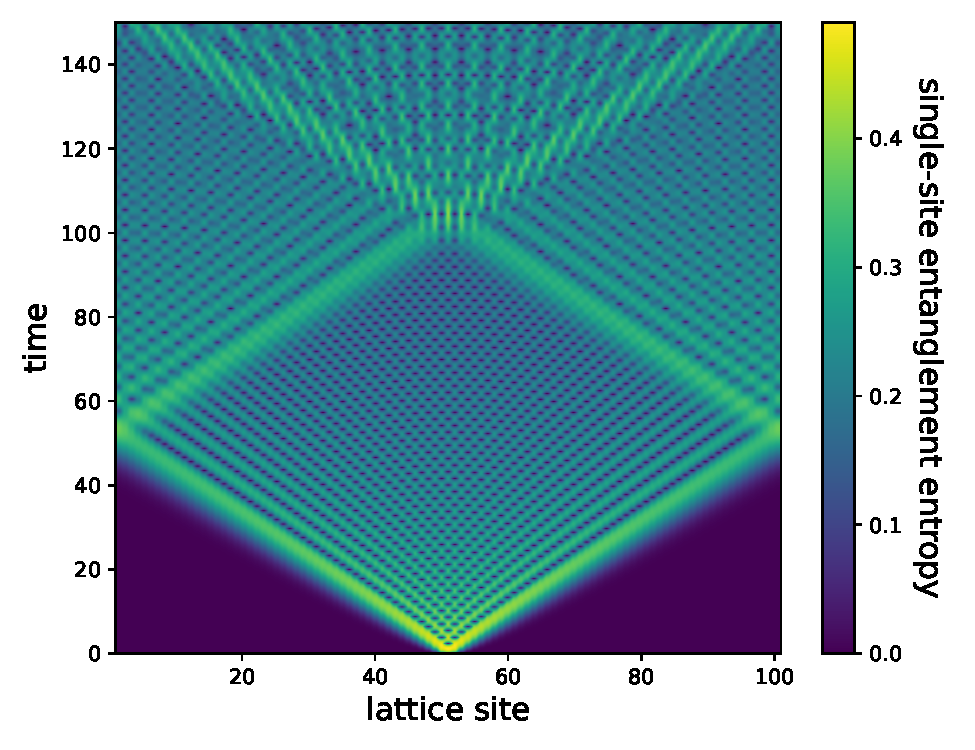
\includegraphics[width=0.3\textwidth]{picture/EntanglementEntropyPropagation_time0.0to150.0_site101.pdf}
  (b)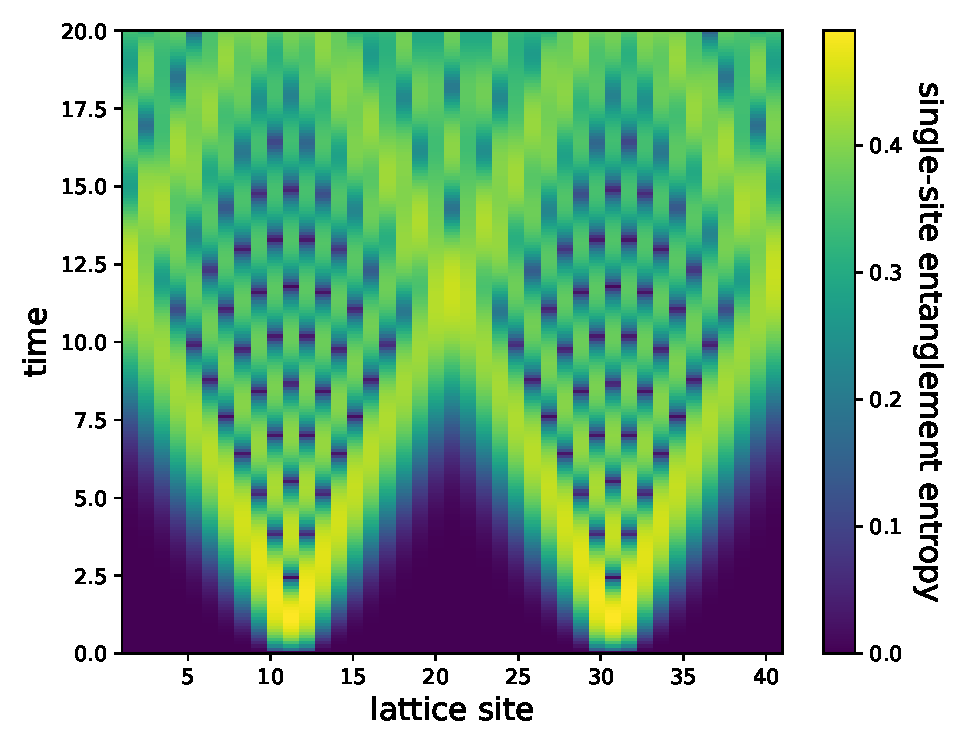
\includegraphics[width=0.3\textwidth]{picture/EntanglementEntropyPropagation_time0.0to20.0_site41_Mtot2.pdf}
  (c)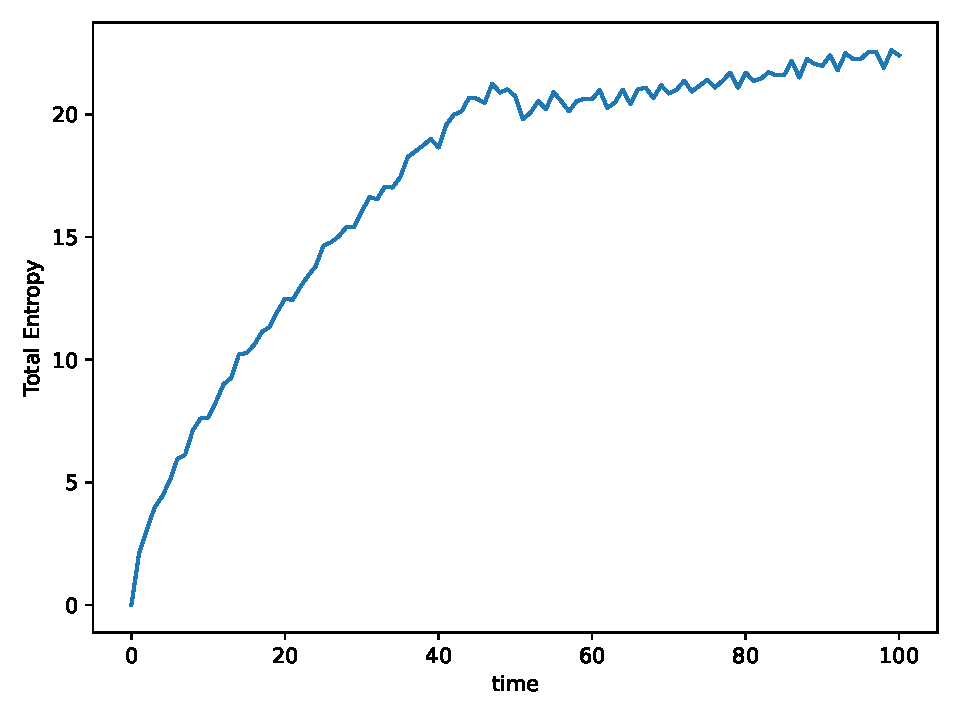
\includegraphics[width=0.3\textwidth]{picture/EntanglementEncreasing_time0.0to100.0_site101}
  \caption{(a) Propagation of single-site entanglement entropy started from a initial state with all spins down and one spin up in the middle. The model Hamiltonian is an one-dimensional Heisenberg spin chain consisting of 100 lattice sites with open boundary condition. (b)  Propagation of single-site entanglement entropy started from a initial state with all spins down but two spins, at the 11th and the 31th site, up. The total number of spins is 40, with open boundary condition. (c)  Growth of total entropy of case (a) as time increases.}\label{fig_propagation-picture}
\end{figure}

\end{document} 